\documentclass[output=paper]{LSP/langsci} 
\ChapterDOI{10.5281/zenodo.1291942}
\renewcommand{\lsChapterFooterSize}{\scriptsize} %footers in editedvolumes
\author{Igor Leturia\affiliation{Elhuyar Foundation}\and Kepa Sarasola\and Xabier Arregi\and Arantza Diaz de Ilarraza\affiliation{\textsc{ixa} Group, University of the Basque Country}\and Eva Navas\and Iñaki Sainz\affiliation{Aholab Group, University of the Basque Country}\and Arantza del Pozo\affiliation{Vicomtech-\textsc{ik}\oldstylenums{4}}\and David Baranda\lastand Urtza Iturraspe\affiliation{Tecnalia}}
\title{The BerbaTek project for Basque: Promoting a less-resourced language via language technology for translation, content management and learning} 
\shorttitlerunninghead{The BerbaTek project for Basque}
\lehead{Leturia, Sarasola, Arregi, Diaz, Navas, Sainz, del Pozo, Baranda \& Iturraspe}
\abstract{Basque is both a minority language (only a small proportion of the population of the Basque Country speaks it) and also a less-resourced language. Fortunately, the Basque regional government is committed to its recovery, and has adopted policies for funding, among other things, language technologies, a field which a language aiming to survive cannot dispense with. BerbaTek was a 3-year (2009--2011) strategic research project on language, speech and multimedia technologies for Basque carried out by a consortium of five members, all prominent local organizations dedicated to research in the above-mentioned areas, and partially funded by the Departments for Industry and Culture of the Basque Government. Collaboration in BerbaTek allowed to carry out a great amount of both basic and applied research. In addition, various prototypes were developed to show the potential of integrating the developed technologies to the language industry sector.}
\maketitle

\begin{document}

 
%i.leturia@elhuyar.com               
%[kepa.sarasola,xabier.arregi,a.diazdeilarraza]@ehu.es
%[eva.navas,inaki.sainz]@ehu.es                  
%adelpozo@vicomtech.org
%[david.baranda,urtza.iturraspe]@tecnalia.com


\section{Introduction}\label{sec:leturia:1}

The Basque language is one of the oldest alive in Europe, although it has suffered continuous regression over the last few centuries. However, many citizens and local or regional governments have been promoting its recovery since the 1970s. Now, Basque holds partial co-official language status in the Basque regions of Spain but it has no official standing in the Northern Basque Country in France, neither in the European institutions. Today, there are about 700,000 Basque speakers, around 25\% of the total population of the Basque Country, but they are not evenly distributed, and the use of Basque in industry and especially in Information and Communication Technology is still not widespread. In September 2012, \textsc{meta-net} placed Basque as one of the 21 European languages that are in danger of digital extinction\footnote{\url{http://www.meta-net.eu/whitepapers/press-release}}. A language that seeks to survive in the modern information society has to be present also in such fields and this calls for language technology products. Basque, like other minority languages, has to make a great effort to address this challenge \citep{WilliamsEtAl2001}. 

In this context, BerbaTek\footnote{\url{http://www.berbatek.com/en}} was a strategic research project in language, speech and multimedia technologies developed over the years 2009--2011. Its consortium was made up of the Elhuyar Foundation, the \textsc{ixa} and Aholab research groups of the \textsc{upv\slash ehu} (University of the Basque Country), the Vicomtech-\textsc{ik}\oldstylenums{4} Visual Interaction and Communication Technologies Centre and the Tecnalia Research \& Innovation foundation. The project was partly funded by the Departments for Industry and Culture of the Government of the Basque Autonomous Community (region of Spain).

The members of the consortium had been collaborating since 2002 in two similar previous projects, Hizking \citep{DiazEtAl2003} and AnHitz \citep{ArrietaEtAl2008}, in which basic foundations, tools and applications were created for Basque.

We believe that research and development for less-resourced languages should be addressing following four points: (1) high standardization, (2) open-source, (3) reuse of language foundations, tools and applications, and (4) incremental design and development. Any \textsc{hlt} project relating to a less-privileged language should follow those guidelines, but from our previous experience we knew that in most cases they did not. We believe that if Basque is now in a fairly good position in \textsc{hlt}, it is because these guidelines have been applied, even though in some cases it was easier to create ``toy'' resources or easily obtainable tools \citep{AlegriaEtAl2011}.

\section{The consortium}\label{sec:leturia:2}

\textit{Vicomtech-\textsc{ik}\oldstylenums{4}}\footnote{\url{http://www.vicomtech.org}} is an applied research center whose main lines of research are graphic computation, interaction and multimedia. Three of its groups participated in BerbaTek: (i) the Speech and \textsc{hlt} group, (ii) the \oldstylenums{3}\textsc{d} Animation group, and (iii) the Audiovisual Content Analysis group.

\textit{Tecnalia}\footnote{\url{http://www.tecnalia.com}} is a private, applied research center specialized in information and telecommunication technologies.

The \textit{Elhuyar Foundation}\footnote{\url{http://www.elhuyar.org}} is a not-for-profit organization, set up with the aim of bringing science and the Basque language together. Elhuyar is firmly established in the market for dictionaries, educational software, multimedia products, plugins and Machine Translation. In 2001, it set up a LT unit.\footnote{\url{http://www.elhuyar.org/hizkuntza-zerbitzuak/EN/R-D}}

\textit{\textsc{ixa}}\footnote{\url{http://ixa.si.ehu.es}} is a group of the University of the Basque Country (\textsc{upv\slash ehu}), consisting of 43 researchers, which works on \textsc{nlp} specialized in the processing of written texts at different levels. The main projects \textsc{ixa} is currently working on are the PATH, OpeNER and NewsReader European STREP projects.

The \textit{Aholab Signal Processing Laboratory}\footnote{\url{http://aholab.ehu.e/}} is a research group of the University of the Basque Country (\textsc{upv\slash ehu}), with broad experience in voice technologies and digital signal processing. Aholab developed the first commercial \textsc{tts} system for Basque, Aho\textsc{tts},\footnote{\url{http://aholab.ehu.es/tts/tts_en.html}} as well as most of the resources and voice processing tools publicly available for Basque.

\section{Objectives}\label{sec:leturia:3}

The main aim of BerbaTek was the research and development of language, speech or multimedia technologies, so that they could provide the technological basis to support the economic sector of the language industries in the Basque Country.

The key challenge was to prove that Basque processing technologies could be useful to improve the performance, social impact and competitiveness of some industrial products. This challenge required the partners to take a new significant step forward in the strengthening of the language industries by incorporating the results and devices into real market scenarios. This point was particularly relevant given that basic resources and tools must be robust enough to support industrial use.

As most companies do not want to take on this task as it is expensive and commercially not profitable, we considered this initiative a social investment. Tools for languages like Basque are usually developed at universities or research centres and adapting those linguistic tools to the real industrial scenario is crucial.

\begin{table} 
\begin{tabularx}{\textwidth}{lX}
\lsptoprule
{Corpus resources} & Basque Dependency Treebank (BDT), 300,000-word corpus.\\
& Basque Propbank and tools for its development \citep{AldezabalEtAl2010}.\\
& AhoSyn, a large speech database (6 hours per speaker) \citep{SainzEtAl2012}.\\
& AhoSpeakers, database designed for voice conversion \citep{SainzEtAl2012}.\\
& AhoEmo3, created for emotional speech synthesis \citep{SainzEtAl2012}.\\
& A large general corpus (+100M words) collected automatically from the web \citep{Leturia2012}.\\
{Ontology resources} & Basque WordNet \citep{PocielloEtAl2011}, the Basque version of WordNet.\\
& \textsc{wnt}erm \citep{PocielloEtAl2008}, WordNet + 25,000 science and technology terms.\\
& Termide, automatic ontology building out of corpora.\\
& QAWS, question answering over Linked Data.\\
{Dictionary resources} & Various bilingual dictionaries created automatically using a pivot language \citep{SaralegiEtAl2012}.\\
\lspbottomrule
\end{tabularx} 
\caption{Resources developed or improved during BerbaTek}
\label{tab:leturia:1}
\end{table}
 

BerbaTek was geared towards applications. Without neglecting basic research, it was endeavouring to present experimental applications which could subsequently be developed further and turned into products by companies. The importance of generating knowledge in the area of language technologies for voice and multimedia lies in their potential for applications mainly in the language industry sector:


\begin{description}
\item[Translation:] interpretation, dubbing, localization, human translation etc.
\item[Content industry:] Internet, audiovisual sector, the media, off- and on-line publishing, multimedia companies, etc.
\item[Training:] language learning, technical and professional education, ongoing 
training, etc.
\end{description}

\newpage 
\section{Resources, tools and applications developed}\label{sec:4}

The partners had been working in \textsc{nlp} and Language Engineering for Basque since 1990. The most basic tools and resources (lemmatizers, \textsc{pos} taggers, lexical databases, speech databases, electronic dictionaries, etc.) had been developed before, but most of them were further improved within the project, and many others were created in BerbaTek. 

\begin{table}
\begin{tabularx}{\textwidth}{lX}
\lsptoprule
{Analysis tools} & Dependency Parsing (\citealt{Bengoetxea2010}; \citealt{AgirreEtAl2011}).\\
& UKB \citep{AgirreSoroa2009} graph-based Word Sense Disambiguation\\
& ArikIturri \citep{Aldabe2010}, automatic creation of exercises out of corpora.\\
{Web as corpus tools} & Co3 \citep{LeturiaEtAl2009}, building multilingual comparable corpora.\\
& PaCo2 \citep{SanVicente2012}, collecting parallel corpora.\\
\lspbottomrule
\end{tabularx}
\caption{Tools developed or improved during BerbaTek}
\label{table:leturia:2}
\end{table}



BerbaTek carried out basic research and built many resources and tools that are necessary for the development of applications. Tables 1, 2 and 3 show the resources, tools and applications developed or improved during the project. The key resources and tools in the development of applications on the aforementioned areas of translation, content management and learning were the following:

\newpage
\begin{itemize}
\item  
Tools for building corpora from the web (monolingual and multilingual, general and domain-based, comparable and parallel), and various corpora collected by using these.
\item 
Syntactic dependency analysers, semantic analyzers and systems for identifying sentence and phrase boundaries.
\item 
Terminology extraction from corpora and automatic building of dictionaries.
\item  
General and domain-specific ontologies and semantic search engines.
\item  
Cross-lingual search and question answering.
\item 
Machine translation systems (rule-based, statistical and hybrid).
\item  
Techniques for voice segment detection and text/image alignment in video.
\item 
Engine for continuous speech recognition; text-to-speech conversion systems.
\item  Speaking avatars.
\item Writing aids and automatic exercise creation.
\end{itemize}
\newpage

\begin{table}[t]\small
  \begin{tabularx}{\textwidth}{lQ}
   \lsptoprule
Automatic dictionary building & AzerHitz \citep{SaralegiEtAl2008}, extraction of equivalent terms from comparable corpora.\\
& PiboLex \citep{SaralegiEtAl2012}, building new dictionaries using a pivot language.\\
& Phraseology and idiomatic expressions extractor \citep{Gurrutxaga2011}.\\
Information retrieval  & Ihardetsi (\citealt{AnsaEtAl2008}; \citealt{AgirreEtAl2009b}), a Question-Answering system.\\
& Elezkari \citep{Saralegi2009}, CLIR (Basque, Spanish and English).\\
Machine translation & Opentrad-Matxin (\citealt{AlegriaEtAl2007}; \citealt{AlegriaEtAl2008}; \citealt{MayorEtAl2011}), open-source rule-based machine translation system for Spanish-Basque.\\
& EU\textsc{smt}, statistical Machine Translation from Spanish to Basque. \citep{Labaka2010}.\\
Speech synthesis & AhoT2P, a letter to allophone transcriber for standard Basque.\\
& Aho\textsc{tts}\_Mod1, a linguistic processor for speech synthesis.\\
& Aho\textsc{tts}, modular Text-To-Speech conversion for Basque, Spanish and English.\\
& \textsc{tts} system based on HTS \citep{ErroEtAl2010}, with own vocoder \citep{ErroEtAl2011a}.\\
& Hybrid Aho\textsc{tts} combining advantages from statistical and unit selection speech synthesis \citep{ErroEtAl2010}.\\
Speech recognition & Aho\textsc{sr} \citep{OdriozolaEtAl2012}, speech recognition engine (standard Basque).\\
\lspbottomrule
\end{tabularx}
\caption{Applications developed or improved during BerbaTek}
\label{tab:leturia:3}
\end{table}

\section{Prototypes}\label{sec:leturia:5}

Throughout the project, we created some demos to show the usefulness of the linguistic tools and the potential of the integration of language-, speech- and multimedia-technologies when it comes to creating applications for the areas of language industries, i.e., for translation, contents and teaching. These are the demos we built:

\largerpage
\begin{itemize}
\item 
Automatic dubbing of documentaries into Basque using subtitles in Spanish (with possible automatic creation of the Spanish subtitles from the Spanish audio, by means of \textsc{asr}).
\item  
Two multimedia and multilingual semantic web search engines on science and technology content, one of them including subsequent navigation through related content or similar images.
\item 
Personal tutor in language learning through a speech-driven avatar, with automatically created grammar and comprehension exercises, writing aids (dictionaries, writing numbers, spelling...) and automatic evaluation of pronunciation.
\end{itemize}

\subsection{Automatic dubbing of documentaries}\label{sec:leturia:5.1}

The automatic dubbing of films is still a difficult challenge (different voices, speed and tones, colloquial language etc.), but for some types of documentaries (single speaker, voice-over, coordination of the lips not necessary or unimportant) we produced a demo that performs satisfactorily. The general structure of the application developed is shown in \figref{fig:leturia:1}. Given a documentary in Spanish and its transcription (the transcription can be obtained automatically by means of any of the available dictation programs for Spanish), Vicomtech-\textsc{ik}\oldstylenums{4}'s alignment technology creates a subtitles file (the transcription with time marks for the beginning and end of each sentence). Then, \textsc{ixa} group's Matxin MT system automatically translates the subtitles into Basque, and Aholab's text-to-speech technology produces the synchronized voice output. We successfully applied this demo to the single-speaker sections of the television programme Teknopolis produced by Elhuyar.

\begin{figure}[h]
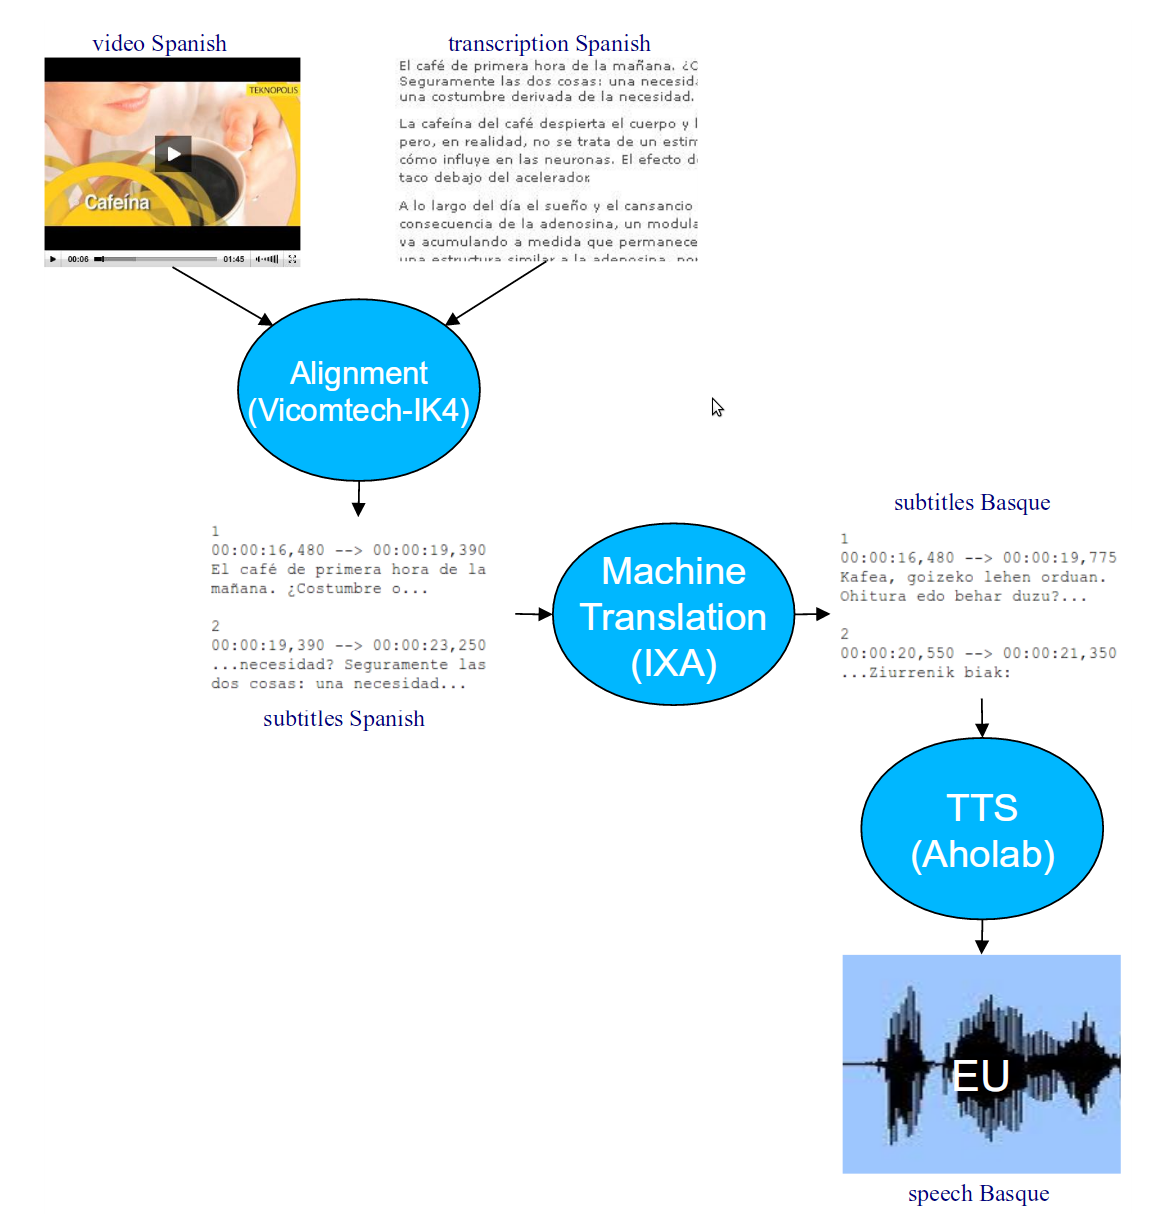
\includegraphics[width=\textwidth]{figures/leturia_1.png}
\caption{Scheme of the automatic dubbing of documentaries demo}
\label{fig:leturia:1}
\end{figure} 

% The demo is online: \url{http://bikoizketaautomatikoa.berbatek.com:8086/demo/en}.  

The automatic alignment of speech and text is based on speech recognition technology. In this case, it is forced to recognize the text of the transcription and provided timing information at phoneme and word levels. That way, the start and end time-codes of each word are obtained automatically and used to synchronize subtitles with the video image.  

The translation of subtitles is done using Opentrad-Matxin \citep{MayorEtAl2011} adapting it to the domain of science and technology. Matxin is a rule-based deep syntactic transfer system for translation into Basque. It translates text from Spanish into Basque, but its architecture allows for an easy implementation of new systems for translating other languages into Basque \citep{Mayor2009}. Opentrad-Matxin is open source. The free code of the Spanish-Basque system with a reduced version of the bilingual lexicon can be downloaded from \url{http://matxin.sourceforge.net}. The system can be used at \url{http://www.opentrad.org}.

The average \textsc{hter} evaluation result of Matxin was 0.42, meaning that 42 editing corrections are required for every 100 tokens. One of the key features of our work is the reuse of existing linguistic resources: we created the system's lexicon by automatically processing high-coverage dictionaries. Given that we reused previously created resources, the \textsc{xml}-based format guaranteed their interoperability. Now we are working on the construction of \textsc{smt} systems and a hybrid system including three subsystems based on different approaches \citep{España-BonetEtAl2011}.

Regarding speech production, we use the \textsc{hmm}-based synthesis  engine. First, its Basque linguistic module extracts linguistic features from the input text. Then the acoustic engine uses them to select previously trained statistical models and generate a sequence of suitable acoustic parameters. 
Finally, the synthetic speech signal is constructed from the aforementioned parameters by AhoCoder. Alignment time stamps are used to synchronize the synthetic audio and the original video, by modifying either the speech rate or the duration of silences.


\subsection{Multimedia and multilingual semantic web search engines}\label{sec:leturia:5.2}
\subsubsection{Semantic retrieval system based on document expansion}\label{sec:leturia:5.2.1}

One of the main problems \textsc{ir} systems have to deal with is the vocabulary mismatch problem between the query and documents: some documents might be relevant for the query even if the specific terms used differ substantially. On the contrary, some documents might not be relevant for the query even if they have some terms in common. The former is because languages are rich in the sense that more than one word or phrase could be used for expressing one idea or thing. The latter is because of ambiguity, in other words, because one word could have more than one interpretation depending on the context. If a system only relies on terms occurring in both the query and the document when it comes to deciding whether a document is relevant, it might be difficult to find some of the interesting documents and also to reject non-relevant documents. It seems fair to think that there will be more chances of successful retrieval if the meaning of the text is also taken into account. Even though this problem has been widely discussed in the literature ever since the early days of \textsc{ir}, it remains unsolved and there is still a high degree of uncertainty about the possibility of overcoming the problem by making use of any \textsc{nlp} technique.

This BerbaTek demo explored whether \textsc{nlp} can benefit the effectiveness of the search engine \citep{Otegi2012}: \url{http://ixa2.si.ehu.es/BerbatekDemo/bilatu}.

Although in principle synonymy, polysemy, hyponymy or anaphora should be taken into account in order to obtain high retrieval relevance, the lack of algorithmic models has prohibited any systematic study of the effect of these phenomena on retrieval. Instead, researchers have resorted to distributional semantic models to try to improve retrieval relevance, and overcome the brittleness of keyword matches. Most research has concentrated on Query Expansion (\textsc{qe}) methods, which typically analyze term co-occurrence statistics in the corpus and in the highest scored documents for the original query in order to select terms for expanding the query terms \citep{ManningEtAl2009}. Document expansion (\textsc{de}) is a natural alternative to \textsc{qe}, but, surprisingly, it has not been explored until very recently. Several researchers have used distributional methods from similar documents in the collection to expand the documents with related terms that do not actually occur in the document. The work carried out in BerbaTek was complementary in that we also explored \textsc{de}, but used WordNet instead of distributional methods \citep{AgirreArregi2010}.

Our key insight was to expand the document with related words according to the background information in WordNet \citep{Fellbaum1998}, which provided generic information about general vocabulary terms. WordNet groups nouns, verbs, adjectives and adverbs into sets of synonyms (synsets), each expressing a distinct concept. Synsets are interlinked with conceptual-semantic and lexical relations, including hyperonymy, meronymy, causality, etc.

In contrast to previous work, we selected those concepts that are most closely related to the document as a whole. For that, we used a technique based on random walks over the graph representation of WordNet concepts and relations. We represented WordNet as a graph as follows: nodes represent concepts (synsets) and dictionary words; relations among synsets are represented by undirected edges, and dictionary words were linked to the synsets associated to them by directed edges. We used version 3.0, with all relations provided, including the gloss relations. This was the setting that achieved the best results in a word similarity dataset \citep{AgirreEtAl2009a}.


Given a document and the graph-based representation of WordNet, we obtained a ranked list of WordNet concepts as follows:

\begin{itemize}
\item 
We first pre-processed the document to obtain the lemmas and parts of speech of the open category words.
\item  
We then assigned a uniform probability distribution to the terms found in the document. The remaining nodes were initialized to zero.
\item 
We computed personalized PageRank \citep{Haveliwala2002} over the graph, using the previous distribution as the reset distribution, and producing a probability distribution over WordNet concepts. The higher the probability for a concept, the more related it was to the given document.
\end{itemize}

This method revealed important concepts, even if they were not explicitly mentioned in the document. Once we had the list of words for document expansion, we created one index for the words in the original documents and another index with the expansion terms. This way, we were able to use the original words only, or to include the expansion words during the retrieval as well.

The retrieval system was implemented using \textsc{mg\oldstylenums{4}j} \citep{Boldi2005}, as it provided state-of-the-art results and allowed several indices over the same document collection to be combined. \textsc{bm\oldstylenums{25}} was the scoring function of choice. It was one of the most relevant and robust scoring functions available \citep{Robertson2009}.


\subsubsection{Multilingual semantic search engine for science and technology based on a specialized ontology, with similar image search}\label{sec:leturia:5.2.2}


As proof of what language technologies could bring to the field of content, we also created a semantic multimedia search engine for science and technology. This search engine is based on the \textsc{wnt}erm ontology \citep{PocielloEtAl2008} specialized in science and technology and created by Elhuyar and \textsc{ixa} (a network in which scientific and technological terms were semantically related to each other, with subclasses, synonyms, etc.), and works on content from Elhuyar (text and images from the Elhuyar magazine, videos from the \textit{Teknopolis} \textsc{tv} show and audio files from the radio programme \textit{Norteko Ferrokarrilla}). Using Tecnalia's technology, the search for a term also shows results containing synonyms, subclasses or superclasses, via the ontology. The resulting search engine is available in two versions, simple and advanced; the advanced version allows to choose an intelligence level (a higher level exploits more the relationships between the concepts in the ontology) and a type of document (image, video, audio and text) and enables filtering by subject. Furthermore, when the result is an image, it shows similar images by means of technology developed at Vicomtech-\textsc{ik}\oldstylenums{4}. A demo is available online at \url{http://bilatzailesemantikoa.berbatek.com/}\href{http://bilatzailesemantikoa.berbatek.com/}. 


One of the first tasks launched was the analysis of the aggregated collection of digital resources made available by the Zientzia.net web site on our semantic search engine site. It was deduced that the Science and Technology domain covered the following subjects: general subjects, computer science, earth science, environment, health, life science, physics, mathematics and chemical science, space and technology in general.

Constructing the BerbaTek ontology included the following steps:

\begin{itemize}
\item 
The manual creation of a skeleton ontology that specified what the root concepts of the ontology were, e.g., Life Science, Technology, Earth science and Computer science. This skeleton should be modified if new knowledge sources were added for the annotation process.

\newpage 
\item 
An ontology with 25,000+ concepts of science and technology was built by hierarchically organizing the terms of the Basque Encyclopaedic Dictionary of Science and Technology produced by Elhuyar. Every term from this ontology, called \textsc{wnt}erm, was mapped to one of the root concepts or areas.
\end{itemize}

\begin{figure}
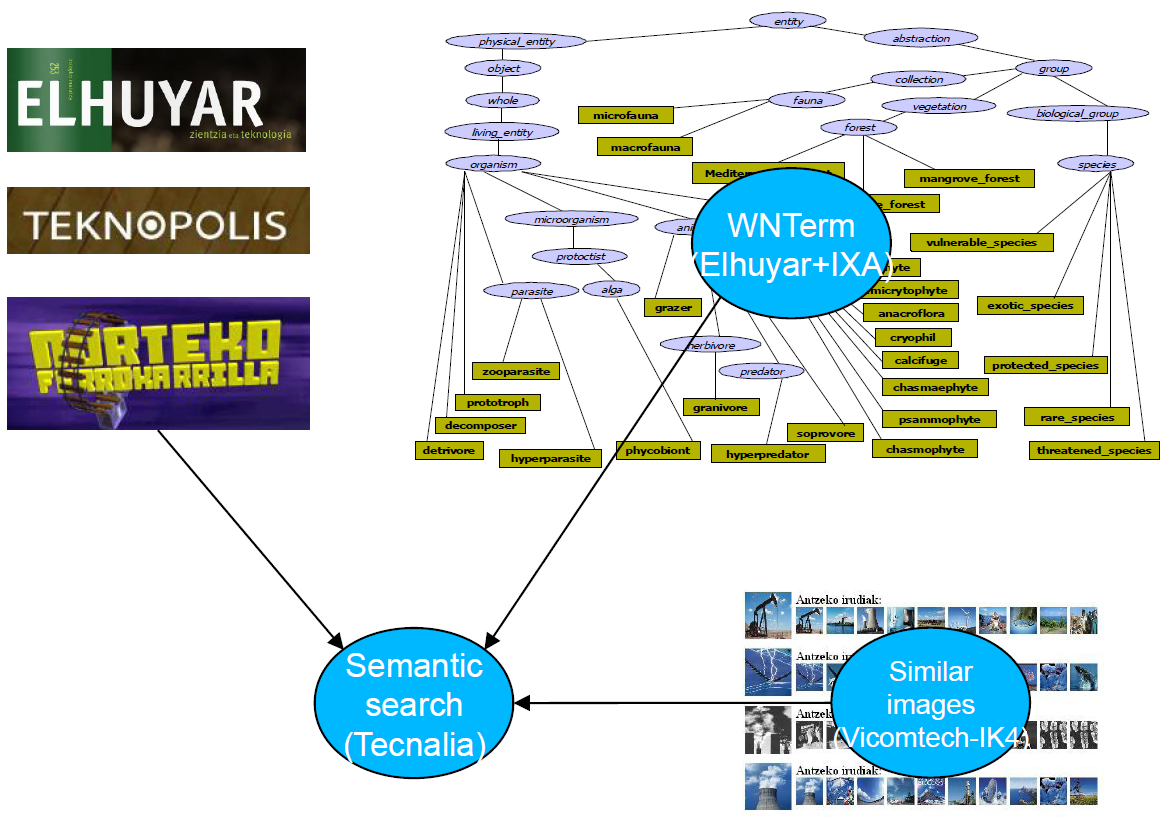
\includegraphics[width=\textwidth]{figures/leturia_2.png}
\caption{Scheme of the semantic search engine demo}
\label{fig:leturia:2}
\end{figure} 

For describing the resources, we decided to adopt an existing and standard metadata model to describe resources, in order to ensure interoperability with other organizations showing interest in sharing resources or contents with our semantic web search engine. Dublin Core was the metadata model selected.

The annotators were provided with a metadata editor where resources could be manually annotated, thus allowing the user to choose the topic or topics for the annotation by selecting from the different predefined concepts in our ontology.

The semantic search engine service was built onto the semantic layer, and we  developed in the service layer the semantic search engine service.

If the search term entered was detected as a concept in the ontology, searches for related concepts were proposed (synonyms, hyponyms, hyperonyms etc.).

If the type of result obtained was an image, the search engine allowed the user to display a list of up to 10 similar pictures. This was because each recorded image had been pre-processed, generating a resemblance relationship.


\subsection{Personal tutor for language learning}\label{sec:leturia:5.3}

For the field of education, we created a demo consisting of a tutor for language learning. This tutor is a \oldstylenums{3}\textsc{d} avatar that showed emotions, developed by Vicomtech-\textsc{ik}\oldstylenums{4}; it speaks Basque and understands what is said in Basque, using Aholab's technology. The tutor assists the student in various tasks: the student can orally solve grammar exercises (verb conjugation, word inflection etc.) and reading comprehension exercises (filling in gaps in a text, multiple choice tests) that are created automatically from texts using technology from \textsc{ixa}; his or her pronunciation can be evaluated with Aholab technology; The tutor can also provide help for writing texts, such as word inflection, writing of numbers or querying dictionaries, by means of technology from \textsc{ixa} and Elhuyar. The technologies included in this demo are shown in \figref{fig:leturia:2}.

The avatar module includes all the necessary functionalities to show and animate the \oldstylenums{3}\textsc{d} character that acts as the front-end of the demo. Its lip animation is synchronized with the audio synthesized by the \textsc{tts} module, and it can also show facial emotions when required. In addition, the module generates blinking and head movement animations through a set of behaviour rules in order to increase the illusion that the \oldstylenums{3}\textsc{d} character is alive. It was developed in \textsc{c++}, using OpenSceneGraph (\url{http://www.openscenegraph.org}) as its graphic library.

\begin{figure}
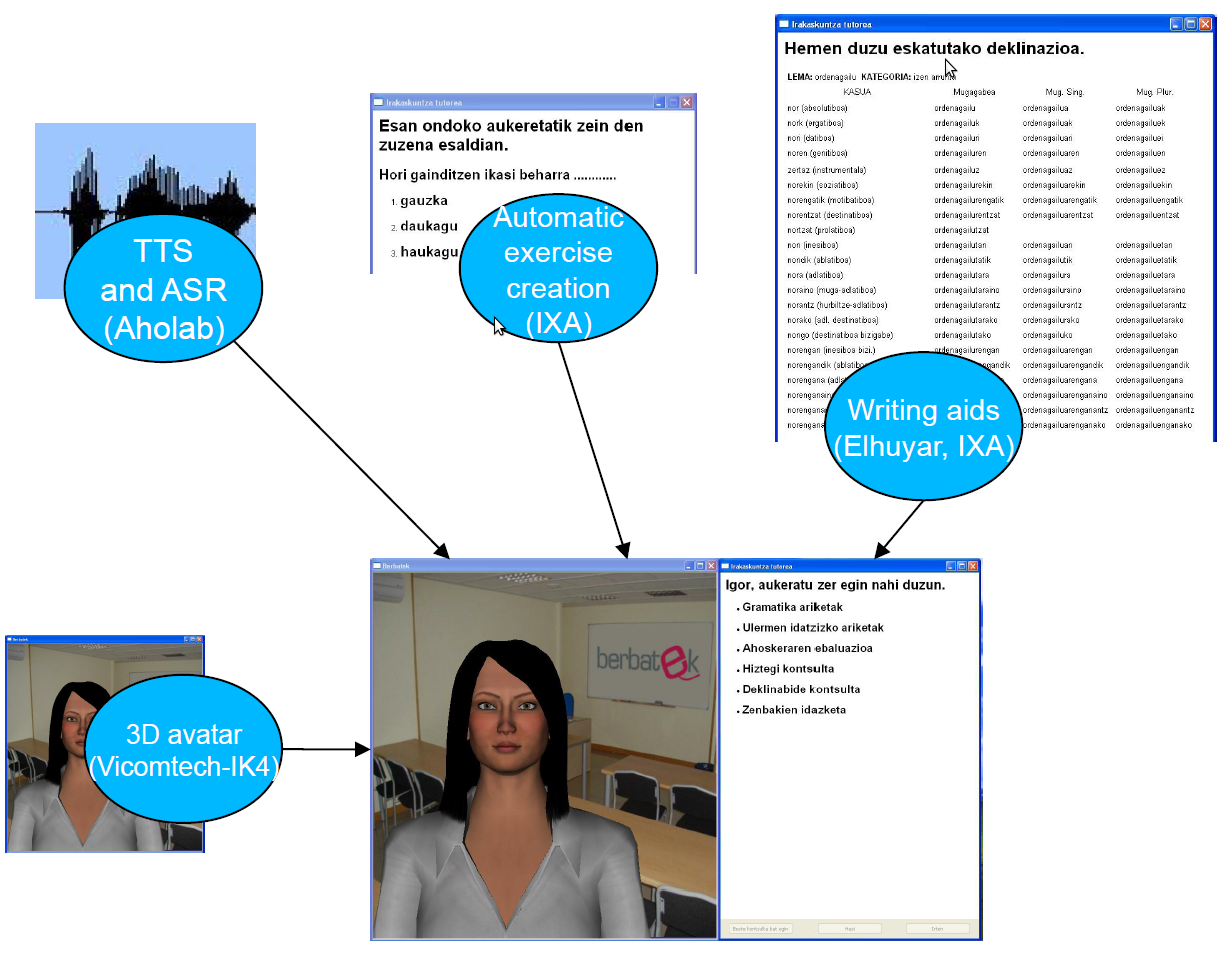
\includegraphics[width=\textwidth]{figures/leturia_3.png}
\caption{Personal tutor in language learning demo}
\label{fig:leturia:3}
\end{figure} 

For the automatic creation of exercises, we use ArikIturri \citep{Aldabe2010}. This is a system for generating different types of questions. It uses as input a set of morphologically and syntactically analyzed sentences represented in \textsc{xml}, and it transforms them into the generated questions, also represented in \textsc{xml}. 

There are some differences between the architecture of our and previous systems (\citealt{KraiftEtAl2004}; \citealt{SchwartzEtAl2004}). We separate an \textit{Answer focus identificator} module and an \textit{Ill-formed questions rejecter} module. \citet{SumitaEtAl2005} also included a module to reject questions, which was based on the web. Depending on the parameters' specifications, the \textit{Sentence retriever} selects candidate sentences from the tagged source corpus. In a first step, it selects the sentences where the specified linguistic phenomena appear. Then the \textit{Candidates selector} studies the percentages of the candidates in order to make a random selection of sentences depending on the number of questions specified in the input parameters. Once the sentences are selected, the \textit{Answer focuses identifier} marks out some of the chunked phrases as answer focuses, depending on the morphosyntactic information of the phrases. Then the \textit{Item generator} creates the questions depending on the specified exercise type. This is why this module contains the \textit{Distractor generator} submodule. By this time, the system has already constructed the question instances. However, as the whole process is automatic, some questions might be ill-formed. That is why we include the \textit{Ill-formed questions rejecter} in the architecture.

With regard to writing aids, the system offers three possible types of help: inflection of words, writing of numbers and querying dictionaries.

The module for helping with inflections asks for a word, then for the case (absolutive, dative, etc.) and then for definiteness and number (singular, plural, indefinite). For the latter two, it can be told to come up with the inflections for all of them. The system calls a web service developed by Elhuyar that generates inflections of words based on a two-level morphology transducer, and returns a table with the inflections of the chosen word.

\newpage 
The writing of numbers module asks for a 1 to 10 suite of one-figure numbers (for example ``\textit{hiru zazpi lau lau bost bat}'', which means ``\textit{three seven four four five one}'') and it tells the user how to write and pronounce the number produced (in the example ``\textit{hirurehun eta hirurogeita hamalau mila, laurehun eta berrogeita hamaika}'', which means ``\textit{three hundred and seventy four thousand, four hundred and fifty one}), using a system developed by Elhuyar.

Finally, the dictionary-querying module asks for a Basque word and looks it up in various online dictionaries produced by Elhuyar (a Basque-Spanish dictionary, a Basque-French dictionary, a Basque-English dictionary and a synonyms dictionary), showing all the results found.

Speech technologies are extensively used in this demo. Aho\textsc{sr}, the \textsc{asr} engine for Basque, is used to recognize the choices and answers of the students, and Aho\textsc{tts} to generate the responses of the avatar. There is also a module to automatically evaluate the correctness of the segmental pronunciation.

The Aho\textsc{tts} version based on \textsc{hmm} is used in this demo. As HTS does not perform any kind of linguistic analysis, the output of the first module of Aho\textsc{tts} has to be translated into proper labels containing phonetic and linguistic information. See \citet{ErroEtAl2010} for a detailed list of the kinds of features encoded into context labels. In order to extract the frame-wise parametric representation of both the spectrum and the excitation, an \textsc{hnm} (Harmonics plus Noise Model)-based vocoder, AhoCoder, is used \citep{ErroEtAl2011b}. This vocoder allows speech to be reconstructed, too. The voice built is a female voice created using a speech database with the same characteristics as the AhoSyn database \citep{SainzEtAl2012}. A female and a male synthetic voice are used in the demo. The female voice is built following the standard procedure, and the male one is obtained by applying voice transformation techniques \citep{ErroEtAl2013}. This Aho\textsc{tts} version is bilingual, works for Spanish and Basque and is available online: \url{http://sourceforge.net/projects/ahotts/}.

Regarding the system that evaluates the correctness of the pronunciation, normally specific databases designed for \textsc{capt} (Computer-Assisted Pronunciation Training) purposes are used. But there is currently no available \textsc{capt} database for Basque. Although there are some speech recognition databases for Basque, the only one which is publicly available \citep{HernáezEtAl2003} was recorded over the fixed telephone network, so it is not suitable for \textsc{capt} purposes, where speech is usually recorded over a microphone. This is why pronunciation teaching systems for Basque have to be developed with other available data. 

The database we use was designed for the training and development of speech recognition for Basque. It is a Speecon-like database \citep{SiemundEtAl2000} and contains recordings from native and non-native speakers, as well as dialectal and standard Basque data for the former. It contains data from a total of 230 speakers, collected in different places of the Basque Country, where Basque has a different official status, health and phonetic influence of neighbouring languages (mainly French and Spanish). During the recording, speakers were asked about their level of language knowledge, so the database could be divided into different subcorpora according to this information. The native speakers' subcorpus was composed of 149 speakers. Non-native speakers spoke Basque as a second language at two different levels: the high level non-natives' subcorpus included 56 speakers and the low level non-natives' subcorpus 25. Due to dialectal variation and also to the different level of fluency, there were some irregularities in the pronunciation of several phonemes, which were not labeled in the transcription. However, they could be partially deduced from the information provided about the speaker. For example, we could obtain information about the region of origin of the speakers and their Basque level through the labels that indicated their city of birth, city of youth and language level. The audio files had their corresponding orthographic transcription file, and the rule-based AhoT2Ptranscriber was used to obtain phonetic transcriptions.

Due to the lack of a suitable speech database with recordings of Basque non-native speakers, the pronunciation evaluation module was developed using a general purpose \textsc{asr} speech database \citep{OdriozolaEtAl2012}. More precisely, the method applied consisted of automatically determining the threshold of \textsc{gop} (Goodness Of Pronunciation) scores, which were used as pronunciation scores at phone-level. Two score distributions were obtained for each phoneme: one corresponding to its correct pronunciation and the other one to its incorrect pronunciation. The distribution of the scores for erroneous pronunciations was calculated artificially by inserting controlled errors in the dictionary, so that each changed phoneme was randomly replaced by a phoneme from the same group. These phoneme groups were obtained by means of phonetic clustering performed by using regression trees. After obtaining both distributions, the \textsc{eer} (Equal Error Rate) of each distribution pair was calculated and used as a decision threshold for each phoneme. The results of the experiments showed that this method was useful even when there was no database specifically designed for \textsc{capt} systems, although it was not as accurate as those specifically designed for this purpose. For the speech recognition module and also for the verification of the correctness of responses, the same database was used.

\section{Conclusions}\label{sec:leturia:6}

Being present in \textsc{ict}s, in general, and in language, speech and multimedia technologies, in particular, is, in our opinion, absolutely necessary for any language that intends to go on living in a world that is becoming more and more mobile, digital and interconnected.

As \citet{AlegriaEtAl2011} stated there is a need of incremental design and development of language resources, tools, and applications in a parallel and coordinated way in order to get the best benefit from them. Our experience in BerbaTek proved that collaboration between research agents working in the aforementioned fields is the right way to go. Apart from doing basic research and developing and putting into the hands of the users a considerable number of basic tools and resources, the integration of the different technologies made it possible to create prototypes of advanced applications for the language industry, i.e., translation, content management and learning. 

The results of the cross-language comparison\footnote{\url{http://www.meta-net.eu/whitepapers/key-results-and-cross-language-comparison}} provided by the \textsc{meta-net} White Paper Series showed that Basque now stands in a better position than some European official languages such as Croatian, Icelandic, Irish, Latvian or Lithuanian; and that Basque is in the 4th among 5 possible levels of support through language technology on Speech, Text Analytics and Languages Resources. The particular White Paper on Basque \citep{HernáezEtAl2012} concluded that there were application tools for speech synthesis, speech recognition, spelling correction, and grammar checking, and that there are also some applications for automatic translation, mainly between Spanish and Basque.

\begin{figure}[h]
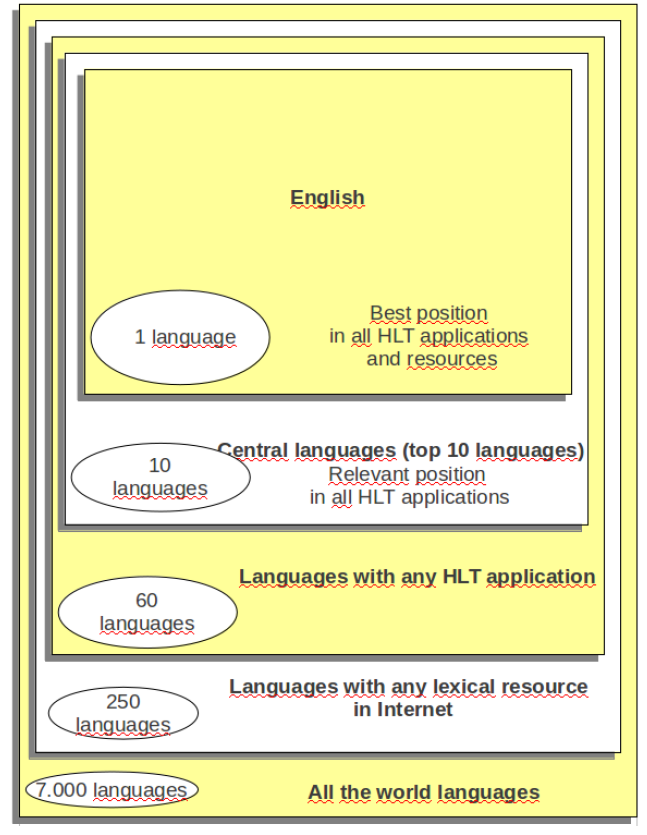
\includegraphics[width=0.5\textwidth]{figures/leturia_4.png}
\caption{Six different levels for less resourced languages}
\label{fig:leturia:4}
\end{figure} 

\figref{fig:leturia:4} shows graphically the classification of the languages in the world  proposed by \citet{AlegriaEtAl2011} according to their degree of development in language technology. As of 2012 Basque is located on an intermediate position in the set of the around 60 languages with some language technology application. It was the 35\textsuperscript{th} language in number of Wikipedia articles. There were 6 products for Basque in the \textsc{elra} catalogue\footnote{\url{http://www.elra.info/}}, 15 products in the \textsc{acl} wiki\footnote{\url{http://aclweb.org/aclwiki/index.php? title=List\_of\_resources\_by\_language}}, and more than 40 on-line dictionaries in the local site hiztegiak.com (although only 5 of them were reflected in yourdictionary.com).

The correlation between Basque speakers and the number of available language products for this language is unusually high. This is due to the coordinated efforts of a few ambitious and productive groups working in successive projects such as BerbaTek. The collaboration of the five main players in Language Technology for Basque in BerbaTek allowed to make a step further in this direction: this cooperation enabled the creation of many new tools and resources and of three new prototypes in the fields of translation, content management and learning.

In the future, we intend to continue our collaboration and move forward with both the basic research and the development of applications and prototypes, for the language industry and also for other fields. But we also intend to go beyond prototypes and, in collaboration with companies devoted to translation, content management and learning, develop and put onto the market real applications for users, which is the next logical step. It will be a challenge that the members of the BerbaTek consortium are willing and prepared to face.

\section*{Acknowledgements}\label{sec:leturia:7}
\largerpage
This research was partially funded by the Regional Government of the Basque Autonomous Community (BerbaTek project, \textsc{\oldstylenums{ie09-262}}) and by the Spanish Ministry of Education and Science (Open\textsc{mt}\oldstylenums{2}, \textsc{tin}\oldstylenums{2009-14675-\textsc{C}03-01}; Know2, \textsc{\oldstylenums{tin2009-14715-C04-01}}; HibridoSint;\textsc{\oldstylenums{tin2010-20218)}}.

\sloppy
\printbibliography[heading=subbibliography,notkeyword=this]

\end{document}
